
%% AHS_2017.tex
%% V1.4b
%% 2015/08/26
%% by Michael Shell
%% See:
%% http://www.michaelshell.org/
%% for current contact information.
%%
%% This is a skeleton file demonstrating the use of IEEEtran.cls
%% (requires IEEEtran.cls version 1.8b or later) with an IEEE
%% conference paper.
%%
%% Support sites:
%% http://www.michaelshell.org/tex/ieeetran/
%% http://www.ctan.org/pkg/ieeetran
%% and
%% http://www.ieee.org/

%%*************************************************************************
%% Legal Notice:
%% This code is offered as-is without any warranty either expressed or
%% implied; without even the implied warranty of MERCHANTABILITY or
%% FITNESS FOR A PARTICULAR PURPOSE! 
%% User assumes all risk.
%% In no event shall the IEEE or any contributor to this code be liable for
%% any damages or losses, including, but not limited to, incidental,
%% consequential, or any other damages, resulting from the use or misuse
%% of any information contained here.
%%
%% All comments are the opinions of their respective authors and are not
%% necessarily endorsed by the IEEE.
%%
%% This work is distributed under the LaTeX Project Public License (LPPL)
%% ( http://www.latex-project.org/ ) version 1.3, and 	may be freely used,
%% distributed and modified. A copy of the LPPL, version 1.3, is included
%% in the base LaTeX documentation of all distributions of LaTeX released
%% 2003/12/01 or later.
%% Retain all contribution notices and credits.
%% ** Modified files should be clearly indicated as such, including  **
%% ** renaming them and changing author support contact information. **
%%*************************************************************************


% *** Authors should verify (and, if needed, correct) their LaTeX system  ***
% *** with the testflow diagnostic prior to trusting their LaTeX platform ***
% *** with production work. The IEEE's font choices and paper sizes can   ***
% *** trigger bugs that do not appear when using other class files.       ***                          ***
% The testflow support page is at:
% http://www.michaelshell.org/tex/testflow/



\documentclass[conference]{IEEEtran}
% Some Computer Society conferences also require the compsoc mode option,
% but others use the standard conference format.
%
% If IEEEtran.cls has not been installed into the LaTeX system files,
% manually specify the path to it like:
% \documentclass[conference]{../sty/IEEEtran}





% Some very useful LaTeX packages include:
% (uncomment the ones you want to load)


% *** MISC UTILITY PACKAGES ***
%
%\usepackage{ifpdf}
% Heiko Oberdiek's ifpdf.sty is very useful if you need conditional
% compilation based on whether the output is pdf or dvi.
% usage:
% \ifpdf
%   % pdf code
% \else
%   % dvi code
% \fi
% The latest version of ifpdf.sty can be obtained from:
% http://www.ctan.org/pkg/ifpdf
% Also, note that IEEEtran.cls V1.7 and later provides a builtin
% \ifCLASSINFOpdf conditional that works the same way.
% When switching from latex to pdflatex and vice-versa, the compiler may
% have to be run twice to clear warning/error messages.






% *** CITATION PACKAGES ***
%
%\usepackage{cite}
% cite.sty was written by Donald Arseneau
% V1.6 and later of IEEEtran pre-defines the format of the cite.sty package
% \cite{} output to follow that of the IEEE. Loading the cite package will
% result in citation numbers being automatically sorted and properly
% "compressed/ranged". e.g., [1], [9], [2], [7], [5], [6] without using
% cite.sty will become [1], [2], [5]--[7], [9] using cite.sty. cite.sty's
% \cite will automatically add leading space, if needed. Use cite.sty's
% noadjust option (cite.sty V3.8 and later) if you want to turn this off
% such as if a citation ever needs to be enclosed in parenthesis.
% cite.sty is already installed on most LaTeX systems. Be sure and use
% version 5.0 (2009-03-20) and later if using hyperref.sty.
% The latest version can be obtained at:
% http://www.ctan.org/pkg/cite
% The documentation is contained in the cite.sty file itself.






% *** GRAPHICS RELATED PACKAGES ***
%
\ifCLASSINFOpdf
\usepackage[pdftex]{graphicx}
  % declare the path(s) where your graphic files are
  % \graphicspath{{../pdf/}{../jpeg/}}
  % and their extensions so you won't have to specify these with
  % every instance of \includegraphics
  % \DeclareGraphicsExtensions{.pdf,.jpeg,.png}
\else
  % or other class option (dvipsone, dvipdf, if not using dvips). graphicx
  % will default to the driver specified in the system graphics.cfg if no
  % driver is specified.
  % \usepackage[dvips]{graphicx}
  % declare the path(s) where your graphic files are
  % \graphicspath{{../eps/}}
  % and their extensions so you won't have to specify these with
  % every instance of \includegraphics
  % \DeclareGraphicsExtensions{.eps}
\fi
% graphicx was written by David Carlisle and Sebastian Rahtz. It is
% required if you want graphics, photos, etc. graphicx.sty is already
% installed on most LaTeX systems. The latest version and documentation
% can be obtained at: 
% http://www.ctan.org/pkg/graphicx
% Another good source of documentation is "Using Imported Graphics in
% LaTeX2e" by Keith Reckdahl which can be found at:
% http://www.ctan.org/pkg/epslatex
%
% latex, and pdflatex in dvi mode, support graphics in encapsulated
% postscript (.eps) format. pdflatex in pdf mode supports graphics
% in .pdf, .jpeg, .png and .mps (metapost) formats. Users should ensure
% that all non-photo figures use a vector format (.eps, .pdf, .mps) and
% not a bitmapped formats (.jpeg, .png). The IEEE frowns on bitmapped formats
% which can result in "jaggedy"/blurry rendering of lines and letters as
% well as large increases in file sizes.
%
% You can find documentation about the pdfTeX application at:
% http://www.tug.org/applications/pdftex
\usepackage{amsmath} % assumes amsmath package installed
\usepackage{amssymb}  % assumes amsmath package installed
\usepackage{balance}
%\usepackage{amsxtra}
%\usepackage{amsfonts}
\usepackage{graphics} % for pdf, bitmapped graphics files
%\usepackage{epsfig} % for postscript graphics files
%\usepackage{float}
\usepackage{graphicx}
%\usepackage{caption}
%\usepackage{setspace}
\usepackage{color}
\usepackage{subfigure}
%\usepackage{subfig}
%\usepackage{psfrag}
%\usepackage{dsfont}
\usepackage{multirow}
%\usepackage{algorithm}
%\usepackage{algorithmic}
\usepackage{todonotes}
\usepackage{url}
\usepackage{hyperref}
\usepackage{bm}


\newcommand{\Ne}{\mathbb {N}}




\usepackage{hyperref}



% *** MATH PACKAGES ***
%
\usepackage{amsmath}
% A popular package from the American Mathematical Society that provides
% many useful and powerful commands for dealing with mathematics.
%
% Note that the amsmath package sets \interdisplaylinepenalty to 10000
% thus preventing page breaks from occurring within multiline equations. Use:
%\interdisplaylinepenalty=2500
% after loading amsmath to restore such page breaks as IEEEtran.cls normally
% does. amsmath.sty is already installed on most LaTeX systems. The latest
% version and documentation can be obtained at:
% http://www.ctan.org/pkg/amsmath
\usepackage{amsthm}

%\usepackage{subcaption}
\usepackage{graphicx}
\graphicspath{ {fig/} }
%\usepackage{subfigure}
% *** SPECIALIZED LIST PACKAGES ***
%
%\usepackage{algorithm}
%\usepackage{algorithmic}
\usepackage[linesnumbered,ruled]{algorithm2e}
% algorithmic.sty was written by Peter Williams and Rogerio Brito.
% This package provides an algorithmic environment fo describing algorithms.
% You can use the algorithmic environment in-text or within a figure
% environment to provide for a floating algorithm. Do NOT use the algorithm
% floating environment provided by algorithm.sty (by the same authors) or
% algorithm2e.sty (by Christophe Fiorio) as the IEEE does not use dedicated
% algorithm float types and packages that provide these will not provide
% correct IEEE style captions. The latest version and documentation of
% algorithmic.sty can be obtained at:
% http://www.ctan.org/pkg/algorithms
% Also of interest may be the (relatively newer and more customizable)
% algorithmicx.sty package by Szasz Janos:
% http://www.ctan.org/pkg/algorithmicx




% *** ALIGNMENT PACKAGES ***
%
%\usepackage{array}
% Frank Mittelbach's and David Carlisle's array.sty patches and improves
% the standard LaTeX2e array and tabular environments to provide better
% appearance and additional user controls. As the default LaTeX2e table
% generation code is lacking to the point of almost being broken with
% respect to the quality of the end results, all users are strongly
% advised to use an enhanced (at the very least that provided by array.sty)
% set of table tools. array.sty is already installed on most systems. The
% latest version and documentation can be obtained at:
% http://www.ctan.org/pkg/array


% IEEEtran contains the IEEEeqnarray family of commands that can be used to
% generate multiline equations as well as matrices, tables, etc., of high
% quality.




% *** SUBFIGURE PACKAGES ***
%\ifCLASSOPTIONcompsoc
%  \usepackage[caption=false,font=normalsize,labelfont=sf,textfont=sf]{subfig}
%\else
%  \usepackage[caption=false,font=footnotesize]{subfig}
%\fi
% subfig.sty, written by Steven Douglas Cochran, is the modern replacement
% for subfigure.sty, the latter of which is no longer maintained and is
% incompatible with some LaTeX packages including fixltx2e. However,
% subfig.sty requires and automatically loads Axel Sommerfeldt's caption.sty
% which will override IEEEtran.cls' handling of captions and this will result
% in non-IEEE style figure/table captions. To prevent this problem, be sure
% and invoke subfig.sty's "caption=false" package option (available since
% subfig.sty version 1.3, 2005/06/28) as this is will preserve IEEEtran.cls
% handling of captions.
% Note that the Computer Society format requires a larger sans serif font
% than the serif footnote size font used in traditional IEEE formatting
% and thus the need to invoke different subfig.sty package options depending
% on whether compsoc mode has been enabled.
%
% The latest version and documentation of subfig.sty can be obtained at:
% http://www.ctan.org/pkg/subfig




% *** FLOAT PACKAGES ***
%
%\usepackage{fixltx2e}
% fixltx2e, the successor to the earlier fix2col.sty, was written by
% Frank Mittelbach and David Carlisle. This package corrects a few problems
% in the LaTeX2e kernel, the most notable of which is that in current
% LaTeX2e releases, the ordering of single and double column floats is not
% guaranteed to be preserved. Thus, an unpatched LaTeX2e can allow a
% single column figure to be placed prior to an earlier double column
% figure.
% Be aware that LaTeX2e kernels dated 2015 and later have fixltx2e.sty's
% corrections already built into the system in which case a warning will
% be issued if an attempt is made to load fixltx2e.sty as it is no longer
% needed.
% The latest version and documentation can be found at:
% http://www.ctan.org/pkg/fixltx2e


%\usepackage{stfloats}
% stfloats.sty was written by Sigitas Tolusis. This package gives LaTeX2e
% the ability to do double column floats at the bottom of the page as well
% as the top. (e.g., "\begin{figure*}[!b]" is not normally possible in
% LaTeX2e). It also provides a command:
%\fnbelowfloat
% to enable the placement of footnotes below bottom floats (the standard
% LaTeX2e kernel puts them above bottom floats). This is an invasive package
% which rewrites many portions of the LaTeX2e float routines. It may not work
% with other packages that modify the LaTeX2e float routines. The latest
% version and documentation can be obtained at:
% http://www.ctan.org/pkg/stfloats
% Do not use the stfloats baselinefloat ability as the IEEE does not allow
% \baselineskip to stretch. Authors submitting work to the IEEE should note
% that the IEEE rarely uses double column equations and that authors should try
% to avoid such use. Do not be tempted to use the cuted.sty or midfloat.sty
% packages (also by Sigitas Tolusis) as the IEEE does not format its papers in
% such ways.
% Do not attempt to use stfloats with fixltx2e as they are incompatible.
% Instead, use Morten Hogholm'a dblfloatfix which combines the features
% of both fixltx2e and stfloats:
%
% \usepackage{dblfloatfix}
% The latest version can be found at:
% http://www.ctan.org/pkg/dblfloatfix




% *** PDF, URL AND HYPERLINK PACKAGES ***
%
%\usepackage{url}
% url.sty was written by Donald Arseneau. It provides better support for
% handling and breaking URLs. url.sty is already installed on most LaTeX
% systems. The latest version and documentation can be obtained at:
% http://www.ctan.org/pkg/url
% Basically, \url{my_url_here}.

% *** Do not adjust lengths that control margins, column widths, etc. ***
% *** Do not use packages that alter fonts (such as pslatex).         ***
% There should be no need to do such things with IEEEtran.cls V1.6 and later.
% (Unless specifically asked to do so by the journal or conference you plan
% to submit to, of course. )


% correct bad hyphenation here
\hyphenation{op-tical net-works semi-conduc-tor}

\newtheorem{problem}{Problem}
\newtheorem{theorem}{Theorem}[section]
\newtheorem{corollary}{Corollary}[theorem]
\newtheorem{lemma}[theorem]{Lemma}
\newcommand*{\affaddr}[1]{#1} % No op here. Customize it for different styles.
\newcommand*{\affmark}[1][*]{\textsuperscript{#1}}
\newcommand*{\email}[1]{\texttt{#1}}

\newcommand\NB[1]{$\spadesuit$\footnote{NB: #1}}
\newcommand\JL[1]{$\diamondsuit$\footnote{MH: #1}}
\newcommand\ME[1]{$\spadesuit$\footnote{ME: #1}}

%\renewcommand{\algorithmicrequire}{\textbf{Input:}}
%\renewcommand{\algorithmicensure}{\textbf{Output:}}
%\newcommand{\algorithmicbreak}{\textbf{break}}
%\newcommand{\BREAK}{\STATE \algorithmicbreak}

%\renewcommand{\baselinestretch}{0.95}

\begin{document}

\title{Cyber-Physical Attack Intention Prediction and System Recovery} 

% affiliations

\author{\IEEEauthorblockN{Mahmoud Elnaggar\affmark[1],
 and Nicola Bezzo\affmark[1,2]}
\IEEEauthorblockA{\affmark[1]Department of Systems and Information Engineering\\
\affmark[2]Department of Electrical and Computer Engineering\\
University of Virginia\\
Email: \{mae3tb,nbezzo\}@virginia.edu}}


% make the title area
\maketitle

% in the abstract
\begin{abstract}
\end{abstract}

% For peer review papers, you can put extra information on the cover
% page as needed:
% \ifCLASSOPTIONpeerreview
% \begin{center} \bfseries EDICS Category: 3-BBND \end{center}
% \fi
%
% For peerreview papers, this IEEEtran command inserts a page break and
% creates the second title. It will be ignored for other modes.
\IEEEpeerreviewmaketitle



\section{Introduction}
Cyber-Physical security has grasped a lot of attention in the research community specially during the last decade. Multiple incidents occured indicate the ability of a malicious attacker to compromise a cyber-physical system through different techniques operating on different levels. For example, The well known cyber attack performed on the Iranian nuclear reactors in 2011 was performed by exploiting five zero-day vulnerabilities in the Operating Systems installed on the computers that operates the SCADA system which controls the nuclear centrifuges. This type of attack operated on the cyber level targeting the physical system by leveraging the knowledge of how the physical system is being operated and controlled by the controllers. Another type of attacks is the one that operates on the system control level, trying to exploit vulnerabilities in the system by compromising different components of the control system.

A typical cyber-physical system consists of the a) controllers b) sensors c) actuators d) the physical system itself. An attacker can compromise the task of the system by attacking any of these components. Attacking sensors can be done in various of ways. One of the most common known attacks on sensors is GPS sensor spoofing, where an attacker can use a hand-held device to deceive the GPS receiver by sending false data. This type of attack if applied to a dynamic cyber-physical system i.e. a UGV or a UAV, it can make the autonomous vehicle to crash or to be hijacked and sent to a desired location.

An example of this type of attacks is the hijacking of the American military drone that was done by Iranians in 2011. The autonomous drone was supposed to land in Afghanistan and the attack sent false positions to the drone via GPS spoofing to deceive the autonomous controller and make it land in Iran instead of Afghanistan. Another example of sensor spoofing attacks was done by researchers from University of Texas and Cornell University, when they conducted an attack by spoofing the GPS receiver on a yakht cruising in the Mediterranean sea which made the yakht go off the desired course while thinking it is still following the correct coarse.\footnote{Motivate that there cyber physical attacks are various and crucial}

Various efforts have been done by members of the research society to maintain the safety of a cyber-physical system by designing systems that are resilient against attacks on sensors. A major contribution was done in solving the problem of secure and resilient state estimation of a cyber-physical system. The results presented in cite show that by using redundant sensors in a system, and leveraging the knowledge of the system model, the secure state estimators are able to correctly estimate the state of the system if the number of attacked sensors is less than half of the number of the sensors.

When resilient state estimator detects an attack, it removes the spoofed of the sensors under attack from the calculations to estimate the state of the system correctly. It doesn't determine whether the attacker was trying to crash the autonomous vehicle into an obstacle or trying to send it to a desired dangerous location. Inferring the intention of the attacker can important for several reasons: In some cases, the identity of the attacker can be revealed which is an important information especially in military applications. Also, inferring the intention of the attacker can be used to predict the future attack vectors on the compromised sensors and therefore, the attack vector can be removed and the compromised sensors can be reused. Another limitation the resilient state estimator has is that considering an attacker that can compromise more than half of the sensors, the resilient state estimator fails to detect which sensors are being compromised and which are not. This urges the need to develop an algorithm that can determine which sensors are being compromised if the system has at least one sensor not being compromised.\footnote{Show the need of attack intention prediction}

In this work, we are interested in addressing the aforementioned issues. We consider the case where we have an autonomous vehicle performing a navigation task and a malicious attacker who can spoof up till N-1 number of sensors. The attacker performs a coordinated attack to send the autonomous vehicle to a desired destination instead of its original destination. The attacker's desired destination can be a hostile territory, or an obstacle the robot will crash by hitting it.

The main contribution of this work is in two folds: First, we leverage Inverse Reinforcement Learning (IRL) techniques to infer the intention of the attacker. In other words, given a set of observations represented by state-action pairs (The states represent the data coming from the sensors, and the actions represent the control input that corresponds to each state), we infer the reward function that the attacker aims to maximize which describes the destination goal the attacker wants the vehicle to go to. Second, we introduce the idea of check-pointing an recovery to a dynamic system under attack. Recording the sensor readings over time can be useful in better detection of attacks that hide within the noise profiles of the sensors. Moreover, by analyzing the history data, we can determine when the attack started and what was the last uncompromised state of the system which can be used to recover the system from the attack by correctly estimating the state of the system.

\subsection{Related Work}\label{subsec:related}
The problem of Inverse Reinforcement Learning has been addressed in multiple domains. It was first introduced by Russel in \cite{Ng2000}. Abbeal and Ng presented an algorithm for apprenticeship learning via IRL  \cite{Abbeel2004a}. They considered the case where the reward function is expressible as a linear combination of known features. Ramachandran et al. \cite{Ramachandran2007} cast the IRL problem as a Bayesian inference problem. They showed that there Bayesian Inverse Reinforcment Learning (BIRL) algorithm can be used for reward learning and also policy learning. They introduced the policy walk algorithm that is based on Monte Carlo Marcov Chain (MCMC) algorithm which is used for sampling. Michini et al. \cite{Michini2015} extended BIRL algorithm to deal with continuous state and action spaces and introduced the Non-Parametric Bayesian Inverse Reinforcement Learning (NBIRL) algorithm.\footnote{To be completed}

The idea of check-pointing and recovery has been applied to many computing systems \cite{Zhang2003,Processors2017,Koo1987, Prakash1996}. By taking snapshots of the state of a system in a cyclic fashion or after the occurrence of specific events, we can roll-back to the last saved checkpoint if a fault occurs to recover the system from that fault. This technique cannot be directly applied to a dynamical system without modifying the definitions of a checkpoint and a roll-back for two reasons. 
\begin{enumerate}
    \item This technique assumes that every checkpoint we take represents a correct state of the system. For a dynamical system under sensor attack, detection of an attack doesn't occur immediately after an attack starts. Which means that the saved checkpoints between the time the attack started and the time it is detected are considered incorrect states. For that matter, we need to consider the fact that we can have correct and incorrect checkpoints in the system and the the recovery mechanism shall find the last correct checkpoint in the system.
    \item Roll-back is considered successful when the last checkpoint is recovered. For a dynamical system which moves in the physical space. To tolerate a fault or mitigate an attack, the recovery process is considered success-full when the correctly estimate the state of the system, not necessarily by returning back to the last saved correct check-point. Thus, the role of the recovery mechanism in our case is to find what is the last correct checkpoint, and use this information to determine the current state of the system correctly.
\end{enumerate}

\section{Preliminaries}\label{sec:Preliminaries}
\subsection{Markov Decision Process}
A finite state Markov Decision Process (MDP) \cite{puterman2014markov} consists of a tuple $(S,A,T,R,\gamma)$ where:
\begin{itemize}
    \item The set $S$ is the set of all the states.
    \item The set $A$ is the set of all possible actions.
    \item The function $T : S\times A\times S \mapsto [0,1]$ is the transition probabilities function. $T(s,a,s')$ is the probability that moving to state $s'$ from state $s$ after action $a$ is taken.
    \item The reward function $R$ can be a function of the state only $R(s)$, a function of states and actions $R(s,a)$, or a function of the states, actions, and the next states $R(s,a,s')$.
    \item The discount factor $\gamma$ is the factor that the reward function gets discounted with over time.
\end{itemize}
To solve and MDP problem, we are interested in finding an optimal stationary policy $\pi^*: S \mapsto A$ that maximizes the expected value of the discounted future rewards.
In order to find $\pi^*$, we need to define a value function for all state $s \in S$ given a reward function $R(s)$ and a policy $\pi$ as follows:
\[ V^\pi(s,R) = R(s) + \sum_{s'}^{}\gamma\,T(s,\pi(s),s')\,V^\pi(s') \]
The value function of state $s$ is equal to the reward received in state $s$ plus the sum of the discounted expected value function for each neighbor state $s'$ when we take actions according to policy $\pi$.
We need also to define a function that evaluates the value of taking action $a$ for each state $s$ which is called the Q-function.
\[Q^\pi(s,a,R) = R(s) + \sum_{s'}{} \gamma\,T(s,a,s')\,V^\pi(s') \]
Then, a policy $\pi$ is optimal iff, for each state $s \in S$:
\[ \pi(s) = \arg\!\max_{a\in A} Q^\pi(s,a,R)\]
The optimal policy $\pi^*$ corresponds to a state value function $V^*$ and a state-action value function $Q^*$.

\subsection{Inverse Reinforcement Learning}
In Inverse Reinforcement Learning (IRL), we consider an agent acting optimally or sub-optimally in an environment; or in MDP terms, the agent is following an optimal or sub-optimal policy $\pi^a(s)$. The policy of the agent $\pi^a(s)$ can be observed as a set of state-action pairs $\mathcal{O} = \{(s_1,a1),(s_2,a_2), ...,(s_N,a_N)\}$. The goal of IRL is to infer the reward function $R(s)$ that is responsible for generating these observations.
\footnote{TODO: Talk about that it is an ill-posed problem ... And previous works made assumptions about the Reward function to solve this problem}

\section{Problem Statement}\label{sec:problem}
We consider an autonomous vehicle (AV) performing a navigation task to a desired destination.  The AV navigates inside an environment The AV has a set of sensors $\mathcal{S}$ where $|\mathcal{S}|=N$, $N$ is the number of AV sensors. We also consider a malicious attacker that can spoof a subset of sensors $\mathcal{S'}$ where $\mathcal{S'} \subset \mathcal{S}$, $|\mathcal{S'}| < N$. The goal of the attacker is to drive the AV towards a hostile destination while hiding the attack within the noise profiles of the spoofed AV sensors. The attack begins at time $t_1$. The attack stays stealthy until the noise margins of the spoofed sensors don't overlap anymore with the noise margins of the uncompromised ones at $t_2$ as shown in Fig. \ref{fig:sensor_spoofing}. From $t_2$, the AV state estimator can detect that there is an attack or fault that led to this divergence in readings, but it cannot distinguish which sensors are compromised and which are not.
\begin{figure}[h]
\caption{An attack on the blue sensor starts at $t_1$. The attack can be detected at $t_2$ when the sensors error margins don't overlap anymore.}
\centering
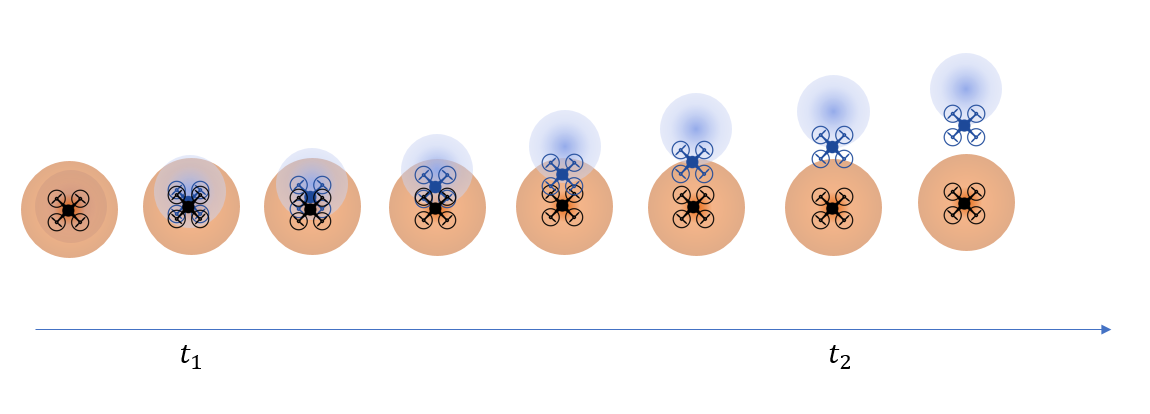
\includegraphics[width=0.5\textwidth]{sensor_spoofing}
 \label{fig:sensor_spoofing}
\end{figure}
We are interested in solving the following two problems:

Problem 1 Attacker Intention Inference: Consider the set $\mathcal{G}$ is the set of states that are considered hostile. Consider a super-set of observations $\mathcal{O}_{t_2:t} = \{\mathcal{O}_1, \mathcal{O}_2, ..., \mathcal{O}_N\}$, where $\mathcal{O}_{i,t_2:t} = \{(s_{i,t_2}, a_{t_2}), (s_{i,t_2+1}, a_{t_2+1}), ..., (s_{i,t_2+t}, a_{t_2+t})\}$ is the finite set of measurement-action pairs for each sensor $i$ which includes the history of sensor data recorded starting from the beginning of the detection time of the attack $t = t_2$ until the current time $t$. We assume the attacker's goal is to drive the AV towards a hostile goal which is located in a position or a state $g^a \in \mathcal{G}$. Where, $\mathcal{G}$ is the set of all possible hostile goals known a priori. Our goal is to infer, at each time t, the intention of the attacker by estimating their desired hostile goal $g^a$ and determine the subset of compromised sensors $\mathcal{S'}$.



Problem 2 Recovery of last safe state:
TO BE MODIFIED
Determining the start time of the attack $t_1$ and the last un-compromised AV state $s_{t_1-1}$ and use this information to recover the actual state of the AV at time $t$.

\section{Attacker Intention Inference}\label{sec:intpredic}
We propose to cast Problem 1 an Inverse Reinforcement Learning problem. In this problem, we consider the compromised AV under attack acts as an agent that navigates in the environment according to a policy $\pi^a$. The policy $\pi^a$ drives the agent towards the hostile destination $g^a$ as fast as possible while hiding the attack within the sensors noise profiles or the environment disturbance model. At each state $s$, the policy $\pi^a$ is calculated according to:
\[ \pi^a(s) = \arg\!\max_{a\in A} Q^{\pi^a}(s,a,R^a)\]

The reward function $R^a$ can take many forms. For the sake of simplicity we assume the reward function $R^a$ that makes the agent moves towards the hostile goal $g$ can be modelled as follows. 
  \begin{equation}
    R^a(s)=\left\{
                \begin{array}{ll}
                  c\hspace{2em} s = g\\
                  0\hspace{2em} s \ne g
                \end{array}
              \right.
  \end{equation}
Where $c$ is a positive constant.

Given the set of observations $\mathcal{O}_{t_2:t}$, the goal is to infer the intention of the attacker by inferring the reward function $R(s)$ the AV is trying to maximize. As attacker can compromise only a subset of sensors $\mathcal{S}'$, we use rely on this assumption to perform attacker's intention inference. Our intuition is that we can use the sensor readings of the compromised set of sensors and the actions taken by the AV to infer that they match the actions of the attacker's policy $\pi_a$. We propose a method that starts examining all the sensor readings and AV actions at the time the attack is detected $t_2$. The goal is to search for the subset of the compromised sensors $\mathcal{S}'$  that cause the AV to drift towards the bad goal. The algorithm we propose leverages Bayesian Inverse Reinforcement Learning techniques (BIRL)\cite{Ramachandran2007} in order to do the inference. In BIRL, the inference of the reward function posterior $Pr(R|O)$ is a function of the reward function prior $Pr(R)$ and the likelihood of the observations $Pr(O|R)$ as follows:
\begin{equation} 
    Pr(R|O) = \frac{Pr(O|R)Pr(R)}{Pr(O)}
\end{equation}
Where, $Pr(O)$ is the probability distribution of $O$ over the entire space of reward function $R$. The normalization constant $Pr(O)$ is usually hard to compute as it requires performing multiple integral calculations which is usually not feasible to compute analytically. To estimate the posterior distribution while avoiding calculating $Pr(O)$, we use the well-known MCMC sampling algorithm. The output of MCMC is an estimate of the distribution of the posterior $Pr(\tilde{R}|O)$. As this is an estimation problem, we are interested reporting the value of $R$ that minimizes the expected Lease Square Error (LSE) of the estimate $E[(R-\tilde{R})^2]$. It is proven in \cite{Ramachandran2007} that the mean of the estimated posterior distribution is the optimal estimator in that case.

In order for the MCMC algorithm to estimate the posterior $Pr(R|O)$, we need to compute two terms in each iteration. The first term is the prior $Pr(R)$ and the second one is the likelihood of the observations $Pr(O|R)$.

The likelihood of the observations can be calculated as follows:
\begin{equation}
Pr(O|R) = \frac{e^{\alpha\sum_{i}{Q^*(s_i,a_i,R)}}}{\sum_{b\in A}{}e^{\alpha\sum_{i}{}Q^*(s_i,b,R)}}
\end{equation}
Where, $\alpha$ is a factor that indicates how much we are confident that the agent is acting optimally. This calculation requires solving MDP problem to compute $Q^*$ for each state-action pairs. This step is computationally expensive and it requires discretization of the state and action spaces which can result in a tremendously sized state space. Inspired by Michini's work in \cite{Michini2013}, we propose to do actions likelihood approximation which doesn't require discretization of the state and action spaces and compute. First, we record the action $a_i$ corresponding to each sensor reading $s_i$ to obtain the necessary set of state-action pairs to perform IRL. Then, to approximate the action likelihood for a goal $g$ at state $s_i$, we compute the difference between action $a_i$ and the action calculated from the controller at state $s_i$ to go to $g$ as follows:
\begin{equation}
P(O_i|R_{g}) = P(a_i|s_i,g) \propto e^{-\alpha \lVert a_i - a_{CL} \rVert_{2}}
\end{equation}
Where $a_{CL}$ is the action given by the system's closed loop controller to go from state $s_i$ to goal $g_i$.

Algorithm 1, shows how we use MCMC for inference.
Initially, we assume that the prior for a hostile goal is normally distributed among all  possible hostile goals. During MCMC iterations we update the for each time step $t$ we run MCMC algorithm to infer the hostile goal of the attacker. We sample a goal $g$ from the set of goals $\mathbb{G}$ and then for each sensor $i$, we compute the posterior of having the goal $g$ as the hostile goal $g_A$ given the set of observations $\mathcal{O}_{i,t_2:t}$ as follows:
\begin{equation} Pr(g=g_a|\mathcal{O}_{i,t_2:t}) \propto Pr(\mathcal{O}_{i,t_2:t} | g = G_A) \\ \times Pr(g=g_a|\mathcal{O}_{i,t_2:t-1})
\end{equation}
The first term on the right hand side of the equation is the likelihood of the observations given that the goal $g$ is the hostile goal $g_A$ which can be computed according to (3) or can be approximated by (4). The second term is the prior which is updated from the posterior calculated at the previous time $t-1$.
By examining all sensor data and all possible bad goals inside the set $\mathcal{G}$, we can infer which set of sensors are compromised and which are not. The recovery part can be done after that by removing the compromised sensors from the state estimator calculations.
\begin{algorithm}
    %\SetKwInOut{Input}{Input}
    %\SetKwInOut{Output}{Output}
    \underline{AIP} ($\mathcal{O}, \mathcal{G}$)\;
    %\Input{Two nonnegative integers $a$ and $b$}
    %\Output{$\gcd(a,b)$}
    \ForEach {$\mathcal{O}_i \subset \mathcal{O} $}
    {
        \While{iteration $t < t_{max}$}{
            \ForEach{Observation $(s_{i,k}, a_k) \in \mathcal{O}_i$}
            { 
                $P(a_k|s_{i,k},g) \leftarrow  e^{-\alpha \lVert a_k - a_{CL} \rVert_{2}}$\;
                $P(g|(s_{i,k}, a_k)) \leftarrow  P(a_k|s_{i,k},g) P(g)$\;
            }
            $g_M \leftarrow mean(P(g|\mathcal{O}_i)$)\;
            \eIf{$g_M \in \mathcal{G}$}
              {
                $g_T \leftarrow g_M$\;
                $z_i \in \mathcal{S}_u$\;
              }
              {
                $z_i \in \mathcal{S}_c$\;
              }
        }
    }
    \caption{Attacker Intention Prediction}
\end{algorithm}
\section{Simulations \& Experimental Results}\label{sec:conclusion}


\section{Conclusions \& Future Work}\label{sec:conclusion}


% conference papers do not normally have an appendix


% use section* for acknowledgment
%\vspace{-15pt}
\section*{Acknowledgment}





% trigger a \newpage just before the given reference
% number - used to balance the columns on the last page
% adjust value as needed - may need to be readjusted if
% the document is modified later
%\IEEEtriggeratref{8}
% The "triggered" command can be changed if desired:
%\IEEEtriggercmd{\enlargethispage{-5in}}

% references section

% can use a bibliography generated by BibTeX as a .bbl file
% BibTeX documentation can be easily obtained at:
% http://mirror.ctan.org/biblio/bibtex/contrib/doc/
% The IEEEtran BibTeX style support page is at:
% http://www.michaelshell.org/tex/ieeetran/bibtex/
%\bibliographystyle{IEEEtran}
% argument is your BibTeX string definitions and bibliography database(s)
%\bibliography{IEEEabrv,../bib/paper}
%
% <OR> manually copy in the resultant .bbl file
% set second argument of \begin to the number of references
% (used to reserve space for the reference number labels box)
\bibliographystyle{IEEEtran}
\bibliography{mendeley}


% that's all folks
\end{document}